\section{Introduction}
\label{sec:intro}

Natural Language Video Localization (NLVL) is a fundamental multimodal understanding task that aims to align textual queries with relevant video segments. NLVL is a core component for various applications such as video moment retrieval \cite{cao_visual_2022}, video question answering \cite{qian_locate_2022,lei_tvqa_2020}, and video editing \cite{gao_end--end_2022}. Prior works have primarily explored supervised 
\cite{zeng_dense_2020, 
wang_temporally_2020, 
soldan_vlg-net_2021, 
liu_context-aware_2021, 
yu_intra-_2020, 
gao_relation-aware_2021} 
or weakly supervised \cite{mun_local-global_2020, zhang_counterfactual_2020, zhang_video_2021} NLVL methodologies, relying on annotated video-query data to various extents.

Obtaining annotated data for NLVL is a labor-intensive process that requires video samples paired with meticulous annotations of video moments and corresponding textual descriptions. Figure \ref{fig:teaser} illustrates the annotation requirements for different levels of supervision in NLVL. Fully supervised methods demand fine-grained moment span annotations, while weakly supervised methods typically rely on query descriptions alone. Nevertheless, both still heavily rely on paired video-language data, which limits practicality in open-domain settings.

\begin{figure}[t!]
    \centering
    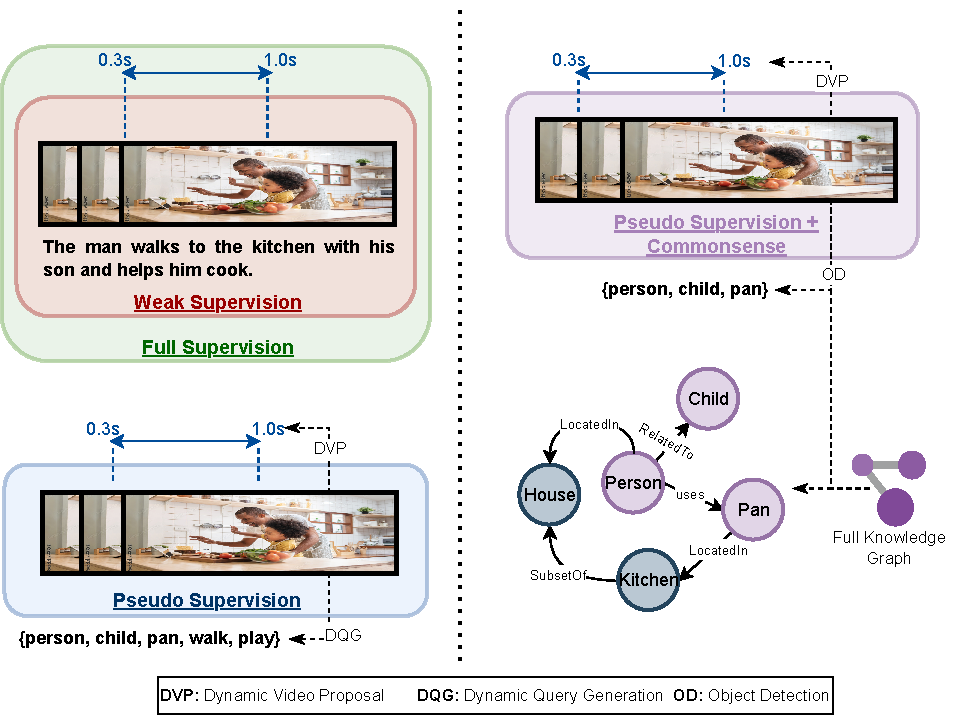
\includegraphics[width=0.9\linewidth]{figures/figure_files/Teaser.pdf}
    \caption{NLVL tasks with different supervision settings.
    Color-coded boxes enclose the annotations components expected at each supervision level. \textbf{\textcolor{ForestGreen}{Full supervision}}: Temporal Video Annotations + Text Queries; \textbf{\textcolor{BrickRed}{Weak Supervision}}: Text Queries; \textbf{\textcolor{Azure}{Pseudo-Supervision}}: Only Raw Videos. Makes use of DVP+DQG; \textbf{\textcolor{Plum}{\modelname~(Ours, right)}} Only Raw Videos. Makes use of DVP+OD and video-informed commonsense knowledge subgraph.}
    \label{fig:teaser}
    
\end{figure}
Recent works formulate zero-shot NLVL, which aims to dynamically generate video moments and their corresponding queries, eliminating the need for paired video-query data \cite{nam_zero-shot_2021,kim2023language}. Nonetheless, existing approaches have certain limitations. On one hand, recent methods generate pseudo-queries using off-the-shelf object detectors for objects (nouns) and text-based language models for actions (verbs), resulting in noisy pseudo-queries that lack grounding in the video content \cite{nam_zero-shot_2021}. On the other hand, language-free methods remove pseudo-queries entirely by utilizing vision-language models pretrained on large-scale image and text datasets \cite{kim2023language}. However, eliminating textual information entirely may lead to missing out on important semantic nuances.

Visual (video) and textual (query) modalities provide very distinct but complementary types of information; videos provide spatial and physical information, while queries provide situational and contextual information. Existing works focus on complex vision-language interactions for observed video-query pairs in an attempt to bridge this gap~\cite{nam_zero-shot_2021,mun_local-global_2020}. However, in the zero-shot/pseudo-supervised setting, where queries are in a simpler form without structural information, finding common ground between modalities becomes crucial for effective cross-modal interactions. Commonsense knowledge, which encompasses general knowledge about the world and relationships between concepts, has proven valuable in various tasks \cite{fang_video2commonsense_2020,ding_dynamic_2021,yu_hybrid_2021,li_representation_2022,maharana_integrating_2021,cao_visual_2022}. By incorporating commonsense information, NLVL models could potentially bridge the semantic gap between video and text modalities, enhancing the cross-modal understanding and performance in zero-shot NLVL.


To this end, this work introduces  \textbf{C}omm\textbf{O}nsense ze\textbf{R}o sh\textbf{O}t la\textbf{N}guage vid\textbf{E}o localiza\textbf{T}ion (\textbf{\modelname}), a zero-shot NLVL model that leverages commonsense knowledge to enhance the pseudo-query generation and cross-modal localization of video moments. We introduce a Commonsense Enhancement Module to enrich the encoded video and query representations with rich contextual information and employ external commonsense knowledge from ConceptNet~\cite{speer_conceptnet_2017} to extract relevant relationships between a predefined set of concepts, mined from the input videos. Our primary objective is to investigate the potential benefits and challenges of leveraging commonsense for zero-shot NLVL. By jointly incorporating commonsense knowledge, we show that our model effectively bridges the gap between visual and linguistic modalities.

The contributions of this work are summarized as follows:
\noindent \textbf{(1)} We introduce \modelname\footnote{Code available at \url{https://github.com/PLAN-Lab/CORONET}}, a zero-shot NLVL framework that utilizes external commonsense knowledge to enrich cross-modal understanding between the visual and natural language components of pseudo-query generation. To the best of our knowledge, we are the first to incorporate commonsense information in zero-shot natural language video localization. 
\noindent \textbf{(2)} \modelname extracts knowledge subgraphs that can be employed to enrich vision-language understanding effectively and an accompanying commonsense enrichment module that can be easily integrated into video localization. 
\noindent \textbf{(3)} We provide empirical evidence of the effectiveness of our approach, demonstrating improvements up to $32.13\%$ across various recall thresholds and up to $6.33\%$ in mIoU. Extensive ablation studies thoroughly investigate the impact of commonsense on zero-shot NLVL performance. 